\chapter{Tips in DL}

\section{Enlarge the FOV}

增加网络的感受野。目前看到的主要方法如下:

\begin{itemize}
\item CRFs\cite{marvin2018crf}
\item Global Graph-reasoning module\cite{chen18iterative}
\item Pooling
\item Dilated conv\cite{YuKoltun2016}
\item 
\end{itemize}


\section{Upsampling}

在卷积以及Pooling之后保持分辨率。目前看到的主要方法如下:

\begin{itemize}
\item Padding
\item Deconvolution
\item Uppooling
\item 
\end{itemize}


\section{Multiscale Ability}

在目标检测(Object Detection)中加入多尺度信息。记得的有以下几个方法:

\begin{itemize}
\item Pyramid Network
\item Stacked CNN ?
\item 
\end{itemize}


\section{Dilated Convolution}

主要原理如下。

\begin{figure}[!hbtp]
\centering
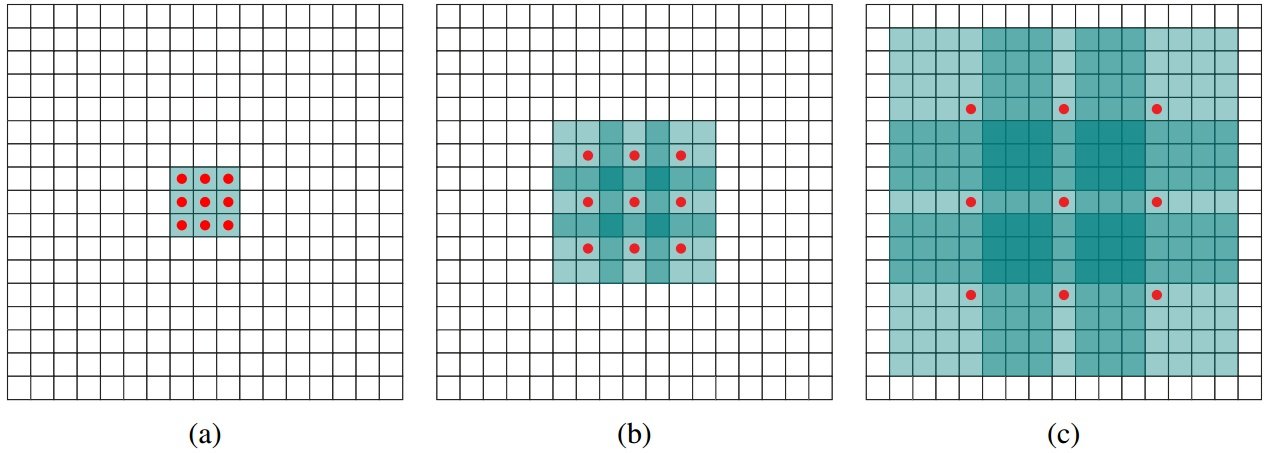
\includegraphics[width=0.75\textwidth]{DLTips/DilatedConv1}
\caption{Dilated Convolution示意图}
\label{DilatedConv1}
\end{figure}

{\bfseries 注意,下文提到的N-Dilated Conv中的$N={1, 2, 3, \ldots}$是指图中相邻红点之间的间隔。}

图\ref{DilatedConv1}中,(a)图对应3x3的1-dilated conv,和普通的卷积操作一样,(b)图对应3x3的2-dilated conv,实际的卷积kernel size还是3x3,但是空洞为1,也就是对于一个7x7的图像patch,只有9个红色的点和3x3的kernel发生卷积操作,其余的点略过。也可以理解为kernel的size为7x7,但是只有图中的9个点的权重不为0,其余都为0。 可以看到虽然kernel size只有3x3,但是这个卷积的感受野已经增大到了7x7{\bfseries(如果考虑到这个2-dilated conv的前一层是一个1-dilated conv的话,那么每个红点就是1-dilated的卷积输出,所以感受野为3x3,所以1-dilated和2-dilated合起来就能达到7x7的conv)},(c)图是4-dilated conv操作,同理跟在两个1-dilated和2-dilated conv的后面,能达到15x15的感受野。对比传统的conv操作,3层3x3的卷积加起来,stride为1的话,只能达到(kernel-1)*layer+1=7的感受野,也就是和层数layer成线性关系,而dilated conv的感受野是指数级的增长。

Dilated的好处是不做Pooling算是信息的情况下,加大了感受野,让每个卷积核输出都包含较大范围的信息。在图像需要全局信息或者语音文本需要较长的Sequence信息依赖的问题中,都能很好的应用Dilated Convolution, 比如图像分割、语音合成WaveNet、机器翻译ByteNet。

WaveNet的例子。
\begin{figure}[!hbtp]
\centering
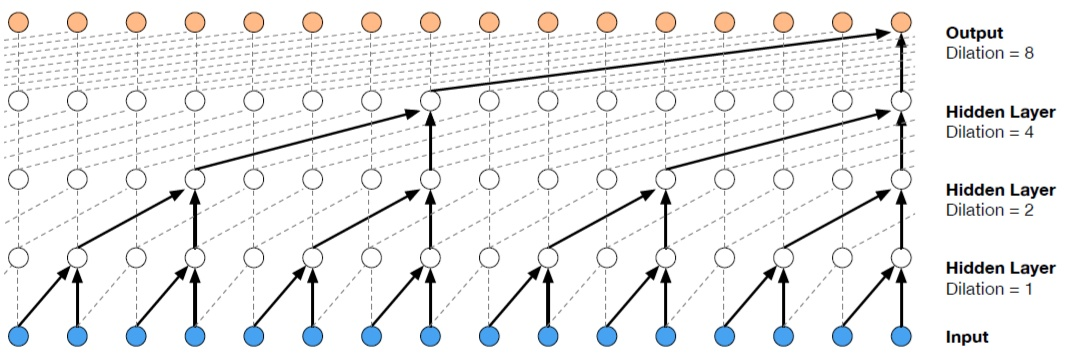
\includegraphics[width=0.75\textwidth]{DLTips/WaveNet1}
\caption{Dilated Convolution在WaveNet中的应用示意图}
\label{WaveNet1}
\end{figure}

参考文献:\href{https://www.zhihu.com/search?type=content\&q=dilated\%20CNN}{Dilated Conv 知乎}

\section{Deconvolutional Network}

参考文献:\href{https://www.zhihu.com/question/43609045/answer/132235276}{Deconvolution Networks}

可能应用的领域:Visualization, Pixel-wise Prediction, Unsupervised Learning, Image Generation.

大致可分为以下几个方面:
\begin{itemize}
\item Unsupervised Learning 

其实是 Covolutional Sparse Coding. 这里的Deconv只是观念上和传统的Conv反向,传统的conv是从图片生成feature map,而deconv是用unsupervised的方法找到一组kernel和feature map,让它们重建图片。

\item CNN Visualization

通过deconv将CNN中conv得到的feature map还原到像素空间,以观察特定的feature map对哪些pattern的图片敏感,这里的deconv其实不是conv的可逆运算,只是conv的transpose,所以tensorflow里一般取名叫transpose\_conv。

\item Upsampling

在pixel-wise prediction比如image segmentation[4]以及image generation[5]中,由于需要做原始图片尺寸空间的预测,而卷积由于stride往往会降低图片size, 所以往往需要通过upsampling的方法来还原到原始图片尺寸,deconv就充当了一个upsampling的角色。

\end{itemize}

下面主要介绍这三个方面的论文。

\subsection{Convolutional Spare Coding}

{\bfseries 第一篇:Deconvolutional Netwoks}

主要用于学习图片的中低层级的特征表示,属于Unspervised Feature Learning。

更多内容参考本小节的参考文献。

\subsection{CNN可视化}
ZF-Net中利用Deconv来做可视化,它是将CNN学习到的Feature Map的卷积核,取转置,将图片特征从Feature Map空间转化到Pixel空间,用于发现哪些Pixel激活了特定的Feature Map,达到分析理解CNN的目的。


\subsection{Upsampling}
用于FCN\cite{Fcn2014}和DCGAN。

\section{Dilated Network与Deconv Network之间的区别}
Dilated Convolution主要用于增加感受野,而不是Upsampling;Deconv Network主要用于Upsample,即增加图像分辨率。

对于标准的$k \times k$的卷及操作,stride为$s$,分为一下几种情况:
\begin{itemize}
\item $s > 1$

即卷积的同时做了降采样,输入Feature Map的分辨率\footnote{分辨率是指像素的多少,而尺度是指模糊程度的大小,即Gaussian Filter中的方差$\delta$}下降。但这一般也会增加感受野。

\item $s = 1$

普通的步长为1的卷积,输入与输出分辨率相同。

\item $\mathbf{0 < s < 1}$

Fractionally strided convolution.相当于图像做upsampling。比如$s=0.5$时,意味着图像像素之间padding一个空白的像素(像素值为0)后,stride改为1进行卷积,达到一次卷积看到的空间范围变大的目的。

\end{itemize}

\section{Uppooling}

In the convnet, the max pooling operation is non-invertible, however we can obtain an approximate inverse by recording the locations of the maxima within each pooling region in a set of switch variables. In the deconvnet, the unpooling operation uses these switches to place the reconstructions from the layer above into appropriate locations, preserving the structure of the stimulus.

也就是说用一组开关变量保存最大值在Pooling Region中的位置。

参考文献: \href{https://www.quora.com/What-is-the-difference-between-Deconvolution-Upsampling-Unpooling-and-Convolutional-Sparse-Coding}{Quora Answer}


\section{目标检测中的mAP的含义}

\begin{itemize}
\item 对于类别C,在一张图像上

首先计算C在一张图像上的精度。

\begin{displaymath}
\label{PrecisionC1}
Precision_C = \frac{N(TP)_C}{N(Total)_C}
\end{displaymath}
其中,$Precision_C$为类别C在一张图像上的精度。$N(TP)_C$为算法检测正确(True Positive)的$C$的个数,检测是否正确按照$IoU > 0.5$算,同理,$T(Total)_C$为这一张图像所有$C$类的个数。所以则一步,仅涉及一个类别$C$以及一张图像。

\item 对于类别C,在多张图像上

这一步计算的是类别$C$的$AP$指数。

\begin{displaymath}
\label{PrecisionC2}
AveragePrecision_C = \frac{\sum Precision_C}{N(TotalImage)_C}
\end{displaymath}
其中,$AveragePrecision_C$是类别$C$的$AP$指数,$Precision_C$为上文计算得到的类别$C$的在一张图像上的精度,然后对所有包含类别$C$的图像上的$C$的精度$Precision_C$求和;$N(TotalImage)_C$为包含类别$C$的图像的数量,也对应于分子中求和所涉及的图像。

\item 在整个数据集上,多个类别

$mAP$在上一步的计算结果的基础上,计算所有类别的$AP$和 / 总的类别数。

\begin{displaymath}
\label{PrecisionC3}
meanAveragePrecision = \frac{\sum_{C} AveragePrecision_C}{N(Class)}
\end{displaymath}
也就是相当于计算所有类别的$\mathbf{AP}$的平均值,是对应于类别总数的平均值。

\end{itemize}

参考文献:\href{https://www.zhihu.com/question/53405779}{知乎文章}

\section{统计学习方法}

一个比较好的总结:\href{http://kubicode.me/2015/08/16/Machine%20Learning/Algorithm-Summary-for-Interview/#SVM%E3%80%81SMO}{机器学习常见算法个人总结}


\section{待续}















